\chapter{評価実験}
\thispagestyle{myheadings}
本システム稼働前の4週間と稼働させた4週間の2つの期間における滞在履歴の比較とアンケートの結果を用いて，このシステムの有効性を評価した．


\section{実験環境}
% BLEビーコン用いてるよ〜もいるね，持ち運び云々で対象外なった人もいる話するなら
% 今回は全体へのアプローチを見るため
我々の研究室で運用されているBLEビーコンを用いた滞在推定システム\cite{staywatch}と入り口付近のみを映したカメラを用いて，研究室に所属する大学生29名を対象に滞在履歴の比較を行った．
この29名は期間内に一度以上滞在履歴が残っており推定に利用するBLEビーコンの電池が切れていない確認が取れた人物を採用した．
被験者には以下のような簡易的な説明のみ行った．
\begin{itemize}
  \item 乗れそうなバスの時刻があれば投票をしてほしい
  \item 車などバスを使用しない場合は帰れそうな時刻に近いものがあれば投票をしてほしい
  \item 実際の投票方法
  \item 投票すると画面に反映される
  \item ダイレクトメッセージが送られる可能性がある
  \item モニターから通知音が鳴る
  \item カメラを設置し確認する
\end{itemize}
研究室で使用頻度の高いテレビの横にモバイルディスプレイを設置し，画面提示を行った．

本実験環境においては，研究室から最寄りのバス停までの徒歩移動に約5〜10分を要すると事前調査により確認されている．
そのため，利用者が会話をしながら移動した場合でも無理なくバスに乗車できる時間として，帰宅推奨時刻に10分を加算した時刻を基準にバスの時刻を選出した．

本研究の実験環境では，帰宅予測時刻の再取得間隔を30分と設定した．
この間隔は，帰宅行動の変化を適切な頻度で反映できる一方で，システム負荷や不要な再計算を抑制できるとして設定したものである．
また，「帰宅が近づいた」と判断する条件を，現在時刻との差が10分以上45分以下の場合と定義し，この条件を満たした場合に時刻の提示を行った
これにより，少なくとも帰宅推奨時刻の15分以上前には情報が提示される設計とした．
% これにより，利用者が提示内容を確認し，投票や退室準備を行うための時間を確保できることを想定している．

さらに，本実験では提示される複数の候補時刻に対する投票締切時刻を，候補時刻のうち最も早い時刻の10分前に設定した．
これは，利用者が投票結果を確認した上で退室準備や移動を開始できる最低限の時間の確保を目的としている．
この締切設定により，投票が実際の帰宅行動に反映されない状況を防ぎ，提示情報の実用性を高める設計とした．

% \section{例題}
\section{滞在履歴の比較}
複数人が共に退室した機会(以下同行機会)と退室同行機会における人数(以下同行人数)の二軸で評価した．

% \section{実行結果}
\subsection{同行機会の比較}% この辺に滞在人数自体の変化に触れる
曜日ごとに1日あたりの同行機会の数を平均し，比較を行ったグラフが図\ref{fig:chance}である．
火曜日が多く日曜日が少ないなど曜日ごとの傾向は確認できた．
これらの傾向は両期間に共通して見られており，システム稼働前後で同行機会数に顕著な差は見られなかった．

\begin{figure}[htb]
  \centering
  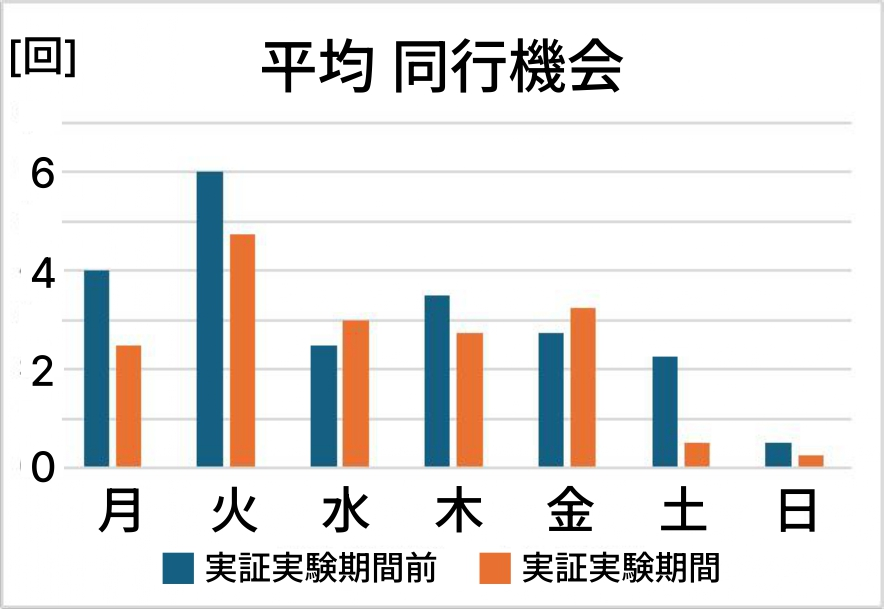
\includegraphics[width=0.6\linewidth]{chance.jpg} % suzuki
  \caption{平均同行機会}
  \label{fig:chance}
\end{figure}

% \subsection{データの登録}
\subsection{同行人数の比較}

曜日ごとに同行機会あたりの人数を平均し，比較を行ったグラフが図\ref{fig:people}である．
$2\sim$3人での同行が多い傾向が見られた．
一方で，システム稼働前後の期間を比較しても，同行人数に顕著な差は確認されなかった．
\begin{figure}[htb]
  \centering
  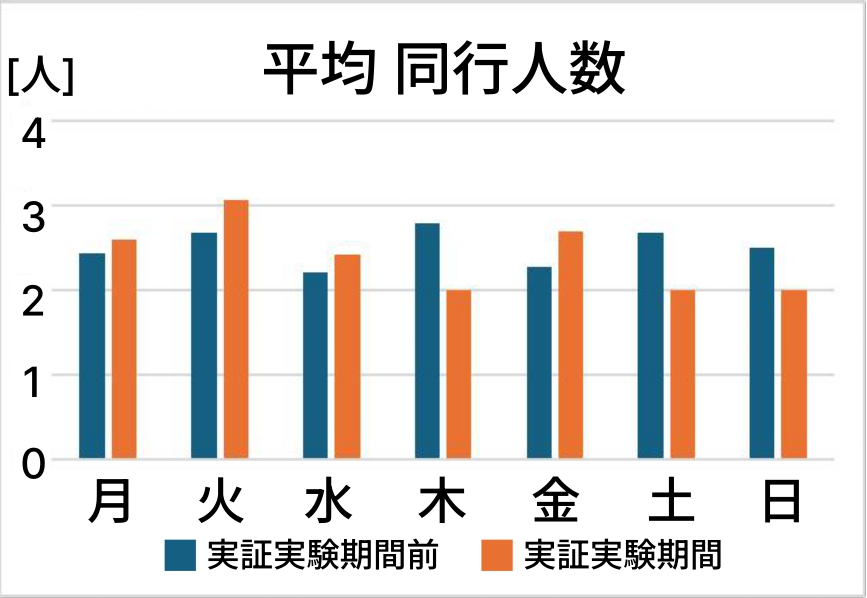
\includegraphics[width=0.6\linewidth]{people.jpg} % suzuki
  \caption{平均同行人数}
  \label{fig:people}
\end{figure}

以上の結果から，同行機会数および同行人数といった定量的指標においては大きな変化は確認されなかったものの，本実験環境における同行行動の基本的な傾向の把握ができた．


\section{アンケート結果}
実験対象である29名にアンケートを実施し，うち19名からシステムの利用率や退室時のコミュニケーションの有効性などについて回答を得た．

\subsection{システムの利用率}
表示時刻に合わせて帰ったかという問いに対して，「ない」「月に一度のみ」「週に一回前後」「それ以上」という選択肢を用意し回答してもらったところ，月に一回以上利用したと答えた人は7人いた．
また，表示時刻を確認してコミュニケーションをとったかという問いに対してリッカート尺度を用いて$1\sim$5で評価してもらった．
回答分布を表\ref{tab:likert}に示す．
回答は1，4，5に多く分布しており，評価が一様ではない点が確認できる．
また，4以上を選択した人は8人おり，平均値は2.7であった．

\begin{table}[htb]
  \centering
  \caption{コミュニケーションに関する評価の回答分布}
  \label{tab:likert}
  \begin{tabular}{c c c c c c}
    \hline
    評価値  & 1 & 2 & 3 & 4 & 5 \\ \hline
    回答人数 & 7 & 2 & 2 & 5 & 3 \\ \hline
  \end{tabular}
\end{table}


%

結果として回答を得た18名のうち3割以上の人が　本システムを実際の帰宅行動やコミュニケーションのきっかけとして活用していたと示唆される．

% \subsection{データの削除}
\subsection{退室時のコミュニケーションの有効性}
期間内か否かに関わらず一緒に退室した際にコミュニケーションは生まれたかという問いに対して，「一人で退室することしかなかった」「一言二言だけ話した」「そのタイミングでのコミュニケーションで仲を深められた」という選択肢を用意し回答を求めた．
「そのタイミングでのコミュニケーションで仲を深められた」と答えた人が9人と最も多く，「一言二言だけ話した」と答えた人が5人とその次に多い．
これは退室時のコミュニケーションへの支援の有効性が示唆される．

\subsection{システム・インタフェースで気になった点}% これ実は考察とがっちゃんこできる？
自由記述により，システム利用時に気になった点について回答を得た．
主な意見として，車を利用する場合のシステムの利用にしにくさ，時刻提示のタイミングが早すぎる，あるいは遅すぎると感じられる場合があるといった意見が得られた．
また，投票状況の視認性やディスプレイサイズに関する指摘も見られた．

\section{考察}
% システムの仕組みや表示が意図を詳細に説明しないとわかりにくかった部分はある
% 実際の環境でも起こりうる話でもあるっちゃあるけど投票率低かった→システムについての説明不足＋プライバシに配慮しすぎて働きかけが弱かった
% ただアプローチ先自体は間違っていなそう，システムが悪いね
本実験では，一定数の被験者が本システムを利用して帰宅行動やコミュニケーションのきっかけとして活用していた一方で，全体としての利用率や投票数は高いとは言えない結果となった．
実際に，帰宅推奨時刻の表示が31回行われたのに対し，投票数の合計は28件にとどまっている．
この要因の一つとして，システムの仕組みや意図が被験者に十分に伝わっていなかった可能性が考えられる．
アンケートの自由記述では，投票の目的や投票結果の扱いについて誤解が見られたと報告されており，提示情報をどのように解釈し，どのように行動すべきかが必ずしも明確でなかったと示唆された．

また，本研究では研究室内での運用を前提とし，被験者の心理的負担やプライバシへの配慮を重視した設計を採用した．
具体的には，個人を強く特定する表現や，投票を強制するような通知は行っていない．
一方で，このような配慮が結果としてシステムからの働きかけを弱め，投票や行動変容につながりにくくなった可能性も考えられる．
アンケートにおいても，表示の存在に気づきにくい，あるいは意図的に気にしなくても目に入るための工夫が欲しいといった意見が見られたので，プライバシ配慮と行動喚起の強度との間には一定のトレードオフが存在すると示唆される．


一方で，アンケート結果からは，退室時というタイミングにおけるコミュニケーションが人間関係の形成や深化につながったと感じている被験者も多く，本研究で対象としたアプローチ先そのものが不適切であったとは言い難い．
これらの結果から，本研究で提案した帰宅タイミングに着目したコミュニケーション支援という考え方は一定の有効性を有している一方で，実運用においてはシステムの提示方法や説明の在り方，および働きかけの強度に関して改善の余地があると考えられる．


% Local Variables: 
% mode: japanese-LaTeX
% TeX-master: "root"
% End: 
